\documentclass[a4paper, 10pt, conference]{ieeeconf}      % Use this line for a4 paper

\IEEEoverridecommandlockouts                              % This command is only needed if 
                                                          % you want to use the \thanks command

\overrideIEEEmargins                                      % Needed to meet printer requirements.

%In case you encounter the following error:
%Error 1010 The PDF file may be corrupt (unable to open PDF file) OR
%Error 1000 An error occurred while parsing a contents stream. Unable to analyze the PDF file.
%This is a known problem with pdfLaTeX conversion filter. The file cannot be opened with acrobat reader
%Please use one of the alternatives below to circumvent this error by uncommenting one or the other
%\pdfobjcompresslevel=0
%\pdfminorversion=4

% See the \addtolength command later in the file to balance the column lengths
% on the last page of the document

% The following packages can be found on http:\\www.ctan.org
%\usepackage{graphics} % for pdf, bitmapped graphics files
%\usepackage{epsfig} % for postscript graphics files
%\usepackage{mathptmx} % assumes new font selection scheme installed
%\usepackage{times} % assumes new font selection scheme installed
%\usepackage{amsmath} % assumes amsmath package installed
%\usepackage{amssymb}  % assumes amsmath package installed
\usepackage{cite}
\usepackage{amsmath,amssymb,amsfonts}
\usepackage{algorithmic}
\usepackage{graphicx}
\usepackage{textcomp}
\usepackage{xcolor}
\usepackage{setspace}
\usepackage{float}
\usepackage{empheq}
\usepackage{newtxmath}  % Times New Roman font for math equations

\title{\LARGE \bf
Environment Similarity Index: Quantifying map-environment divergences for robot localization performance estimation and improvement
}


\author{Christian Rosendahl Dam$^{1}$, Daniel Suvei$^{2}$ and Leon Bodenhagen$^{3}$% <-this % stops a space
\thanks{*This work has been funded by the Danish Innovation Fund.}% <-this % stops a space
\thanks{$^{1}$Christian Rosendahl Dam is with University of Southern Denmark,
        The Maersk Mc-Kinney Moller Institute,
        Odense, Denmark
        {\tt\small chrdam@mmmi.sdu.dk}}%
\thanks{$^{2}$Daniel Suvei is with Teradyne Robotics,
        Odense, Denmark
        {\tt\small dsu@mir-robots.com}}%
\thanks{$^{3}$Leon Bodenhagen is with University of Southern Denmark,
        The Maersk Mc-Kinney Moller Institute,
        Odense, Denmark
        {\tt\small lebo@mmmi.sdu.dk}}%
}


\begin{document}

\maketitle
\thispagestyle{empty}
\pagestyle{empty}


% ----------------------------------------- ABSTRACT --------------------------------------------------

\begin{abstract}
        Should take about this much space: \newline
        abc abc abc abc abc abc abc abc abc abc abc abc abc abc abc abc abc abc abc abc abc abc abc abc abc abc abc abc abc abc abc abc abc abc abc abc abc abc abc abc abc abc abc abc
        abc abc abc abc abc abc abc abc abc abc abc abc abc abc abc abc abc abc abc abc abc abc abc abc abc abc abc abc abc abc abc abc abc abc abc abc abc abc abc abc abc abc abc abc
        abc abc abc abc abc abc abc abc abc abc abc abc abc abc abc abc abc abc abc abc abc abc abc abc abc abc abc abc abc abc abc abc abc abc abc abc abc abc abc abc abc abc abc abc
        abc abc abc abc abc abc abc abc abc abc abc abc abc abc abc abc abc abc abc abc abc abc abc abc abc abc abc abc abc abc abc abc abc abc abc abc abc abc abc abc abc abc abc abc. 
\end{abstract}

% ----------------------------------------- INTRODUCTION --------------------------------------------------

\section{INTRODUCTION}

Robust, lifelong localization is a fundamental ability for all Autonomous Mobile Robots (AMRs). For many years, the gold standard to achieve this has been to use some variation 
of Monte Carlo Localization, as it strikes a good balance between cost and performance. It can perform global localization, and is multi-modal. For indoor industrial applications, 
it works well in many cases. It does however, have a major drawback: It assumes the environment is static. As soon as it' surroundings have changed too much, the particle filter 
diverges and fails, because it does not update it's representation. Making a system that is robust to change is still an ongoing challenge (ref). Some would argue that 
Simultaneous Localization and Mapping (SLAM) is the best way to solve this; but SLAM suffers in reliability. No system is perfect, and sooner or later, an error will find its way 
into the system. The resulting erroneous pose will propagate into the resulting map, reducing accuracy or cause a complete loss of localization. Since there is no ground truth 
to inform the system when the errors was introduced, it is impossible to recover the last valid map state. Therefore, this paper suggests a different approach; instead of updating 
the map, the environment is analysed to detect changes between what is seen and what is expected. This info is then used to alter the behavior of the localization system 
- in this case, adaptive MCL (AMCL). To do this, we need a metric that defines how similar (or different) the observed environment is from its representation (the map). 
However; to the best of our knowledge, no such metric exists. We hypothesize that such a metric can be used to infer the performance of any given localization module that takes 
the static world assumption, and that it can be used online to adjust its behaviour, thereby reducing the pose error. Furthermore, it can be used to generate a heatmap of 
an environment, which can then be interpreted by a human operator, in order to identify local regions of high divergence. These are the contributions of this paper:

We propose the Environment Similarity Index (ESI): An index that quantifies how well the currently observed environment matches the map.
We also show how the ESI correlates to changes in the environment, both on simulated and real-world data, and how these changes impacts AMCL's performance. 
In addition, we show how the ESI can be used by a user to easily identify areas in their site that have changed since mapping, and therefore may increase localiztion errors. 
Finally, we show how the ESI can be used to improve AMCL's performance by using it to dynamically tune AMCL's parameters.

\section{Related Work}
- Bayes filtering / Probabilistic map update
- Scan-BIM divergences
- Occupancy grid vs feature maps
- 

% ----------------------------------------- METHODOLOGY --------------------------------------------------

\section{Methodology}
This section describes how changes in the environment are defined, and how they are used to calculate the ESI.
\subsection{Changes}
The difference that is measured is defined as a \textit{change in how the robot perceives its environment}. The change is measured against the map the robot has of said environment. 
This is an important definition, with three major aspects. The first is that there can be a lot of changes to an environment, but if the robot does not sense it, then the changes 
by definition have no impact on the robot's ability to localize itself. 
The second is that it makes the index agnostic to which localization method is used, and which sensor modalities are available. A difference in observed visual features (I.e. SIFT) 
can be used just as well as geometric lidar, radar or sonar points, both 2D and 3D. The third is that changes that *could* be sensed but aren't, should not affect the index. 
Changes that happen outside the sensor coverage can naturally not be detected, and so they have no effect on localization. Unseen changes may also change back to the initial state 
before they are even noticed. The metric should as mentioned apply to any kind of sensors used, but since MiR robots localize via 2D Lidar, this will be the sensor modality used 
from here on. The reference map could likewise be of any kind (graph based, geometry based, grid based, etc), but for this project, the (occupancy) grid-based map is selected. 

Any physical object can result in a change in the environment by being either removed, added, moved, deformed or alter how it interacts with the sensor. 
However, this can be simplified to just Removed and Added. Any of the last three changes (moved, deformed, different sensor interaction) can be considered as a combination 
of removing the original item, and adding in the new. The distinction makes no difference from the robots point of view. Finally, an object can be observed to be 
exactly as expected - this will be denoted as Matched. There are many ways a sensor reading can be categorized as either of these, and the method chosen is by no means 
the only viable option. 

\subsection{The Environment Similarity Index (ESI)}
The index is a ratio, based on the current pose estimate from the robots localization module - for this paper, AMCL. On every laser-scan callback, each ray point is evaluated: 
Is it close to an expected obstacle in the map? If yes, count as a \underline{Matched}. If not, count as an \underline{Added}. This tells us that an object has been added to the environment 
that is not on the map.  In addition, all laser rays that returned a value are traced in the map from the scanner and outwards to detect obstacles that they \textit{should} 
have hit but didn't. These objects count towards \underline{Removed} to indicate that something on the map has been removed from the environment. 
These classifcations are then used to calculate the ESI score; Figure X provides an overview of the classification.

\begin{figure}[htbp]
    \centerline{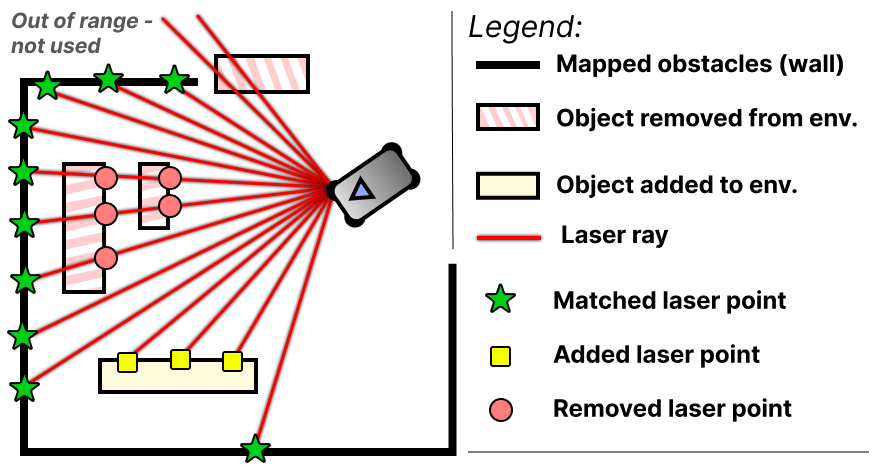
\includegraphics[width=\columnwidth]{figures/figure_1_esi_example.png}}
    \caption{Example of a figure caption.}
    \label{fig1}
\end{figure}

\subsection{Formal Definition}
\textbf{Matched:}
Let $S$ be a 1D vector representing a single scan containing $n_s = |S|$ geometric scan points $s: S = (s_0, s_1, \dots, s_{n_s-1})$.
Only scan points that return a value within min and max range are considered valid. The points are indexed by $i$ where $0 \le i < n_s$.
Let $G$ be a 1D vector representing the discrete geometric reference map, flattened from its original $N$-dimensional form:

$G = (g_0, g_1, \dots, g_{n_g-1})$
The occupancy value at index $i$ is $v(g_i)$, which equals 1 if $g_i$ represents an obstacle, and 0 otherwise.
The assignment $\lambda(i)$ returns the index in $G$ with the shortest distance to the scan point $s_i$:
\begin{equation}
\lambda(i)=\underset{0\le j<n_g}{\text{arg min }}d(s_i,g_j)
\end{equation}
The distance $d(p_1, p_2)$ is the Euclidean distance between two points in $R^N$, where $N$ depends on the map representation, but any distance metric can be used.
Let $T$ be a variable distance threshold. It is based on the expected yaw noise $\gamma$ [rad] and the range of the scan point $r(s_i)$:
\begin{equation}
T(i)=\sin(\gamma)*r(s_i)
\end{equation}
Define a match as:
\begin{equation}
\chi_M(i) = \begin{cases} 1 & \text{if } d(s_i, g_{\lambda(i)}) < T(i), \\ 0 & \text{otherwise}. \end{cases}
\end{equation}
The number of matches for a single scan is then:
\begin{equation}
M = \sum_{i=0}^{n_s-1} \chi_M(i)
\end{equation}

\textbf{Added:}
All valid scan points are classified as either Match or Added. Therefore, the number of added is simply the number of valid scan points minus the number of matches:
\begin{equation}
A = n_s - M
\end{equation}

\textbf{Removed:}
Each valid scan point defines the endpoint of a line from the scanner to that point, as seen in the world frame.
The laser ray $L$ contains all the discrete map points in $G$ that lie on that line:
$L = (l_0, l_1, \dots, l_{n_r-1})$ where $l_0$ is closest to the scanner.
We define a removed point to be every rising edge (going from free to occupied) that the ray encounters from the scanner and out.
Define removed as:
\begin{equation}
\chi_R(j) = \begin{cases} 1 & \text{if } v(l_j) = 1 \text{ and } v(l_{j-1}) = 0 \\ 0 & \text{otherwise}. \end{cases}
\end{equation}
The count of removed items (first encounters) in a scan with $k$ rays is then:
\begin{equation}
R = \sum_{k}\sum_{j=1}^{n_r^{(k)}-1} \chi_R^{(k)}(j)
\end{equation}

\textbf{ESI:}
The ESI score for a single scan S is then defined as:
\begin{equation}
ESI \in [0,1] = \frac{M}{M+A+R}
\end{equation}
and since $n_s = M + A$, the final expression becomes:
\begin{equation}
ESI = \frac{\sum_{i=0}^{n_s-1}\chi_M(i)}{n_s+\sum_{k}\sum_{j=1}^{n_r^{(k)}-1} \chi_R^{(k)}(j)}
\end{equation}

If the scan only sees matches, the ratio is 1/1 = 1, indicating a perfect match with the map.
Both added and removed points increases the denominator equally, driving the index down.  
Note how this reflects reality; there is no upper limit to how much you can change an environment; you can always use a sensor 
with a greater range and higher resolution and then add more items that are not mapped. 
The index therefore converges towards zero as more changes are made, but it will only be exactly zero if it sees zero matches.
The index can be calculated for any number of measurements per sensor update, and can be used for any given localization module. 

% ----------------------------------------- EXPERIMENTS --------------------------------------------------


\section{Experiments}
In this section, we describe the two experiments designed demonstrate how the ESI can be used to:
\begin{itemize} 
\item Quantify and visualize changes in the environment, and to what degree it accurately reflects these changes.
\item Estimate and predict AMCL's performance in rapidly changing environments.
\item Reduce AMCL's pose estimation error in rapidly changing environments by dynamically tuning its parameters.
\end{itemize}

\subsection{Real-world experiment} 
To demonstrate that the ESI works on a real robot in a real enviroment, and that it can be used to visualize changes in it, we used a MiR100 AMR as the platform.
The venue is the production hall of a packaging and labeling company. It is chosen because it represents the type of environment where AMCL often struggles;
it is constantly developing, and most of the time, the the majority of what the robot is able to see consists of transient objects, as seen in Figure X. \newline
\textbf{Setup:} A small section of the hall is mapped, using the native mapping functionality (based on ROS1 cartographer). We placed two waypoints, A and B in it.
The task of the robot is simply to move between them. 

\begin{figure}[H]
    \centerline{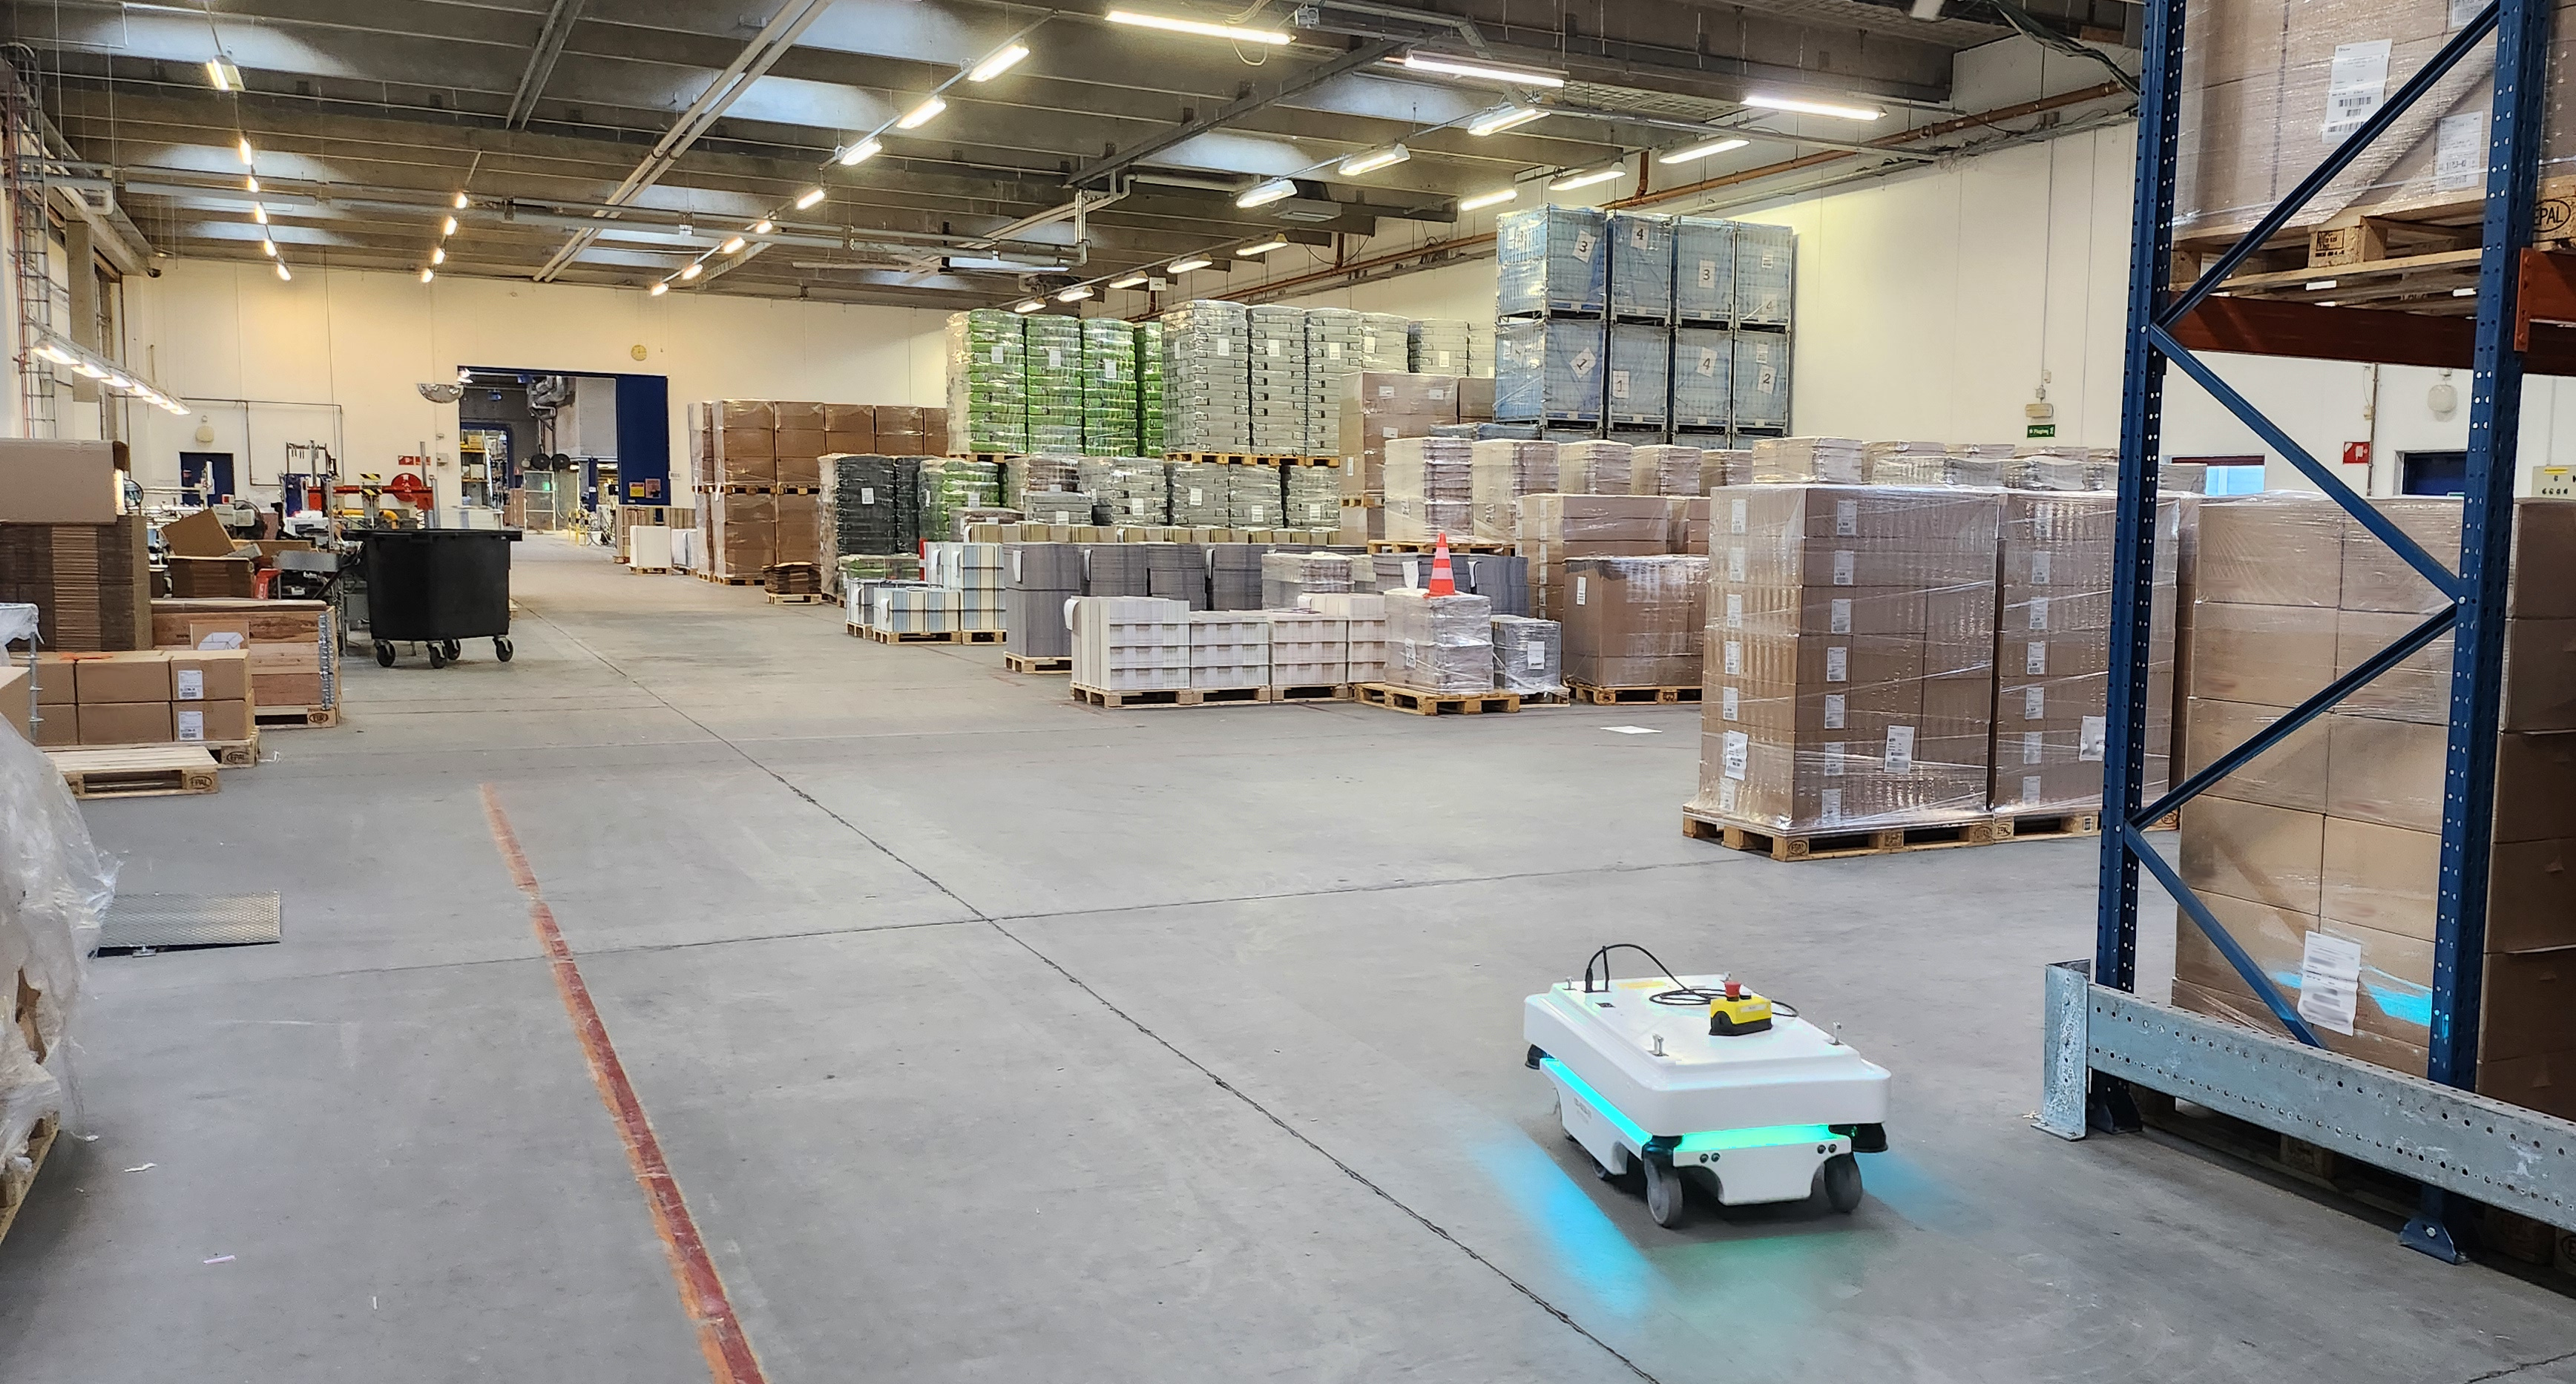
\includegraphics[width=\columnwidth]{figures/schur_img_1.png}}
    \caption{Example of a figure caption.}
    \label{fig2}
\end{figure}



\subsection{Simulation experiment}
...

\section{Conclusions}
...

\section{Limitations and Future work}
...

\subsection{Figures and Tables}

\begin{table}[h]
\caption{An Example of a Table}
\label{table_example}
\begin{center}
\begin{tabular}{|c||c|}
\hline
One & Two\\
\hline
Three & Four\\
\hline
\end{tabular}
\end{center}
\end{table}


   \begin{figure}[thpb]
      \centering
      \framebox{\parbox{3in}{We suggest that you use a text box to insert a graphic (which is ideally a 300 dpi TIFF or EPS file, with all fonts embedded) because, in an document, this method is somewhat more stable than directly inserting a picture.
}}
      %\includegraphics[scale=1.0]{figurefile}
      \caption{Inductance of oscillation winding on amorphous
       magnetic core versus DC bias magnetic field}
      \label{figurelabel}
   \end{figure}
   

\section{CONCLUSIONS}

A conclusion section is not required. Although a conclusion may review the main points of the paper, do not replicate the abstract as the conclusion. A conclusion might elaborate on the importance of the work or suggest applications and extensions. 

\addtolength{\textheight}{-12cm}   % This command serves to balance the column lengths
                                  % on the last page of the document manually. It shortens
                                  % the textheight of the last page by a suitable amount.
                                  % This command does not take effect until the next page
                                  % so it should come on the page before the last. Make
                                  % sure that you do not shorten the textheight too much.

%%%%%%%%%%%%%%%%%%%%%%%%%%%%%%%%%%%%%%%%%%%%%%%%%%%%%%%%%%%%%%%%%%%%%%%%%%%%%%%%



%%%%%%%%%%%%%%%%%%%%%%%%%%%%%%%%%%%%%%%%%%%%%%%%%%%%%%%%%%%%%%%%%%%%%%%%%%%%%%%%



%%%%%%%%%%%%%%%%%%%%%%%%%%%%%%%%%%%%%%%%%%%%%%%%%%%%%%%%%%%%%%%%%%%%%%%%%%%%%%%%
\section*{APPENDIX}

Appendixes should appear before the acknowledgment.

\section*{ACKNOWLEDGMENT}


% ----------------------------------------- REFERENCES --------------------------------------------------


\newpage
\begin{thebibliography}{00}
\bibitem{b1} M. Young, The Technical Writer's Handbook. Mill Valley, CA: University Science, 1989.
\bibitem{b2} J. Doe, A. Smith, and B. Johnson, ``Lorem ipsum dolor sit amet, consectetur adipiscing elit,'' in Proc. IEEE Int. Conf. Robotics Automat., 2020, pp. 123--128.
\bibitem{b3} C. Williams, D. Brown, and E. Davis, ``Sed do eiusmod tempor incididunt ut labore,'' IEEE Trans. Robot., vol. 35, no. 4, pp. 456--467, Aug. 2019.
\bibitem{b4} F. Miller, G. Wilson, and H. Taylor, ``Ut enim ad minim veniam, quis nostrud exercitation,'' in Proc. IEEE/RSJ Int. Conf. Intell. Robots Syst., 2021, pp. 234--241.
\bibitem{b5} I. Anderson, J. Martinez, and K. Lee, ``Ullamco laboris nisi ut aliquip ex ea commodo consequat,'' IEEE Robot. Automat. Lett., vol. 6, no. 2, pp. 789--795, Apr. 2021.
\bibitem{b6} L. Garcia, M. Rodriguez, and N. Patel, ``Duis aute irure dolor in reprehenderit,'' in Proc. IEEE Int. Conf. Robot. Automat., 2018, pp. 567--574.
\bibitem{b7} O. Thompson, P. White, and Q. Harris, ``In voluptate velit esse cillum dolore eu fugiat,'' IEEE Trans. Automat. Sci. Eng., vol. 17, no. 3, pp. 1234--1245, Jul. 2020.
\bibitem{b8} R. Clark, S. Lewis, and T. Walker, ``Nulla pariatur excepteur sint occaecat cupidatat,'' in Proc. IEEE Conf. Decision Control, 2019, pp. 345--352.
\bibitem{b9} U. Young, V. Hall, and W. Allen, ``Non proident, sunt in culpa qui officia deserunt,'' IEEE Trans. Syst., Man, Cybern., Syst., vol. 50, no. 8, pp. 2345--2356, Aug. 2020.
\bibitem{b10} X. King, Y. Wright, and Z. Scott, ``Mollit anim id est laborum,'' in Proc. IEEE Int. Conf. Robotics Automat., 2022, pp. 678--685.
\bibitem{b11} A. Adams, B. Baker, and C. Carter, ``Sed ut perspiciatis unde omnis iste natus error,'' IEEE Robot. Automat. Mag., vol. 27, no. 2, pp. 89--97, Jun. 2020.
\bibitem{b12} D. Evans, E. Foster, and F. Green, ``Sit voluptatem accusantium doloremque laudantium,'' in Proc. IEEE/RSJ Int. Conf. Intell. Robots Syst., 2020, pp. 456--463.
\bibitem{b13} G. Hill, H. Jackson, and I. Jones, ``Totam rem aperiam, eaque ipsa quae ab illo inventore,'' IEEE Trans. Robot., vol. 36, no. 5, pp. 1234--1245, Oct. 2020.
\bibitem{b14} J. Kelly, K. Lopez, and L. Moore, ``Veritatis et quasi architecto beatae vitae dicta sunt,'' in Proc. IEEE Int. Conf. Robot. Automat., 2021, pp. 789--796.
\bibitem{b15} M. Nelson, N. Owens, and O. Parker, ``Explicabo nemo enim ipsam voluptatem quia voluptas,'' IEEE Robot. Automat. Lett., vol. 5, no. 4, pp. 2345--2352, Oct. 2020.
\bibitem{b16} P. Quinn, R. Reed, and S. Ross, ``Sit aspernatur aut odit aut fugit, sed quia consequuntur,'' in Proc. IEEE Conf. Decision Control, 2020, pp. 567--574.
\bibitem{b17} T. Stewart, U. Turner, and V. Underwood, ``Magni dolores eos qui ratione voluptatem sequi nesciunt,'' IEEE Trans. Automat. Sci. Eng., vol. 18, no. 2, pp. 3456--3467, Apr. 2021.
\bibitem{b18} W. Vance, X. Vega, and Y. Vincent, ``Neque porro quisquam est, qui dolorem ipsum quia dolor sit amet,'' in Proc. IEEE Int. Conf. Robotics Automat., 2019, pp. 890--897.
\bibitem{b19} Z. Ward, A. Watson, and B. Webb, ``Consectetur, adipisci velit, sed quia non numquam eius modi tempora,'' IEEE Trans. Syst., Man, Cybern., Syst., vol. 51, no. 6, pp. 4567--4578, Jun. 2021.
\bibitem{b20} C. West, D. Wood, and E. Wright, ``Incidunt ut labore et dolore magnam aliquam quaerat voluptatem,'' in Proc. IEEE/RSJ Int. Conf. Intell. Robots Syst., 2021, pp. 123--130.
\bibitem{b21} F. Yang, G. Young, and H. Zhang, ``Ut enim ad minima veniam, quis nostrum exercitationem ullam corporis,'' IEEE Robot. Automat. Mag., vol. 28, no. 3, pp. 123--134, Sep. 2021.
\bibitem{b22} I. Zhao, J. Zhou, and K. Zhu, ``Suscipit laboriosam, nisi ut aliquid ex ea commodi consequatur,'' in Proc. IEEE Int. Conf. Robot. Automat., 2020, pp. 234--241.
\bibitem{b23} L. Abbott, M. Bell, and N. Cooper, ``Quis autem vel eum iure reprehenderit qui in ea voluptate velit esse,'' IEEE Trans. Robot., vol. 37, no. 1, pp. 5678--5689, Feb. 2021.
\bibitem{b24} O. Davis, P. Edwards, and Q. Ellis, ``Quam nihil molestiae consequatur, vel illum qui dolorem eum fugiat,'' in Proc. IEEE Conf. Decision Control, 2021, pp. 345--352.
\bibitem{b25} R. Fisher, S. Ford, and T. Fox, ``Quo voluptas nulla pariatur at vero eos et accusamus,'' IEEE Robot. Automat. Lett., vol. 6, no. 3, pp. 6789--6796, Jul. 2021.
\bibitem{b26} U. Grant, V. Gray, and W. Green, ``Et iusto odio dignissimos ducimus qui blanditiis praesentium,'' in Proc. IEEE Int. Conf. Robotics Automat., 2021, pp. 456--463.
\bibitem{b27} X. Hayes, Y. Hughes, and Z. Hunt, ``Voluptatum deleniti atque corrupti quos dolores et quas molestias,'' IEEE Trans. Automat. Sci. Eng., vol. 19, no. 1, pp. 7890--7901, Jan. 2022.
\bibitem{b28} A. Ingram, B. Irwin, and C. Irwin, ``Excepturi sint occaecati cupiditate non provident, similique sunt in culpa,'' in Proc. IEEE/RSJ Int. Conf. Intell. Robots Syst., 2022, pp. 567--574.
\bibitem{b29} D. Jenkins, E. Jensen, and F. Johnson, ``Qui officia deserunt mollitia animi, id est laborum et dolorum fuga,'' IEEE Trans. Syst., Man, Cybern., Syst., vol. 52, no. 4, pp. 2345--2356, Apr. 2022.
\bibitem{b30} G. Klein, H. Knight, and I. Knox, ``Et harum quidem rerum facilis est et expedita distinctio,'' in Proc. IEEE Int. Conf. Robot. Automat., 2022, pp. 678--685.

\end{thebibliography}




\end{document}
